\part{Technical Description}\label{part:tech}

\chapter{Website's Structure}\label{chap:structure}

This section will describe the different parts of the website, from the Home page (Sec. \ref{fig:home_page}) and its Menu (Sec. \ref{sec:structure_menus}) leading to the Meta-category (Sec. \ref{sec:structure_metacategories}) and Category (Sec. \ref{sec:structure_categories}) pages (with the special case of the Language category (Sec. \ref{sec:structure_language}). Then the section will describe the Posts (Sec. \ref{sec:structure_post}) and the pages generated automatically by its tags and categories (Sec. \ref{sec:structure_auto}) and will finish by explaining the General Information menu (Sec. \ref{sec:structure_genaralinfo}).

\section{Home page}\label{sec:structure_home_page}

The home page\footnote{Home page: \href{https://ippog-resources-portal.web.cern.ch/}{https://ippog-resources-portal.web.cern.ch/}} is the first page the user gets to. It aims to present the website and redirect to the main pages of the website. A screenshot is available in Figure \ref{fig:home_page}.

\subsection*{a. Home banner}
[Cover block] including the logo of the IPPOG Collaboration with a catchphrase "Explore the foundations of the universe!" over a picture of students participating in International Physics Masterclass.

\subsection*{b. Title}
[H1 Title block]: "Presenting Particle Physics Outreach Projects".

\subsection*{c. Presentation}
[Paragraph block] presenting the website.

\subsection*{d. Meta-Categories}
[Paragraph block] introducing the categories followed with [Buttons block] leading to the meta-categories pages nested within [Cover block] in a [Columns block].

\subsection*{e. Latest entries}
[Title H2] Block followed by a [News block]\footnote{The News block is a CERN customized Query Loop displaying posts and allowing the filtering per categories and/or tags. The choice was made to display the image, title, tags and excerpt of posts.} displaying the 3 latest articles uploaded. Note that it is possible to force the displayed articles as their uploaded date can be updated.

\subsection*{f. Footpage banner}
[Cover block] following the IPPOG color chart.

\begin{figure}[p]
    \centering
    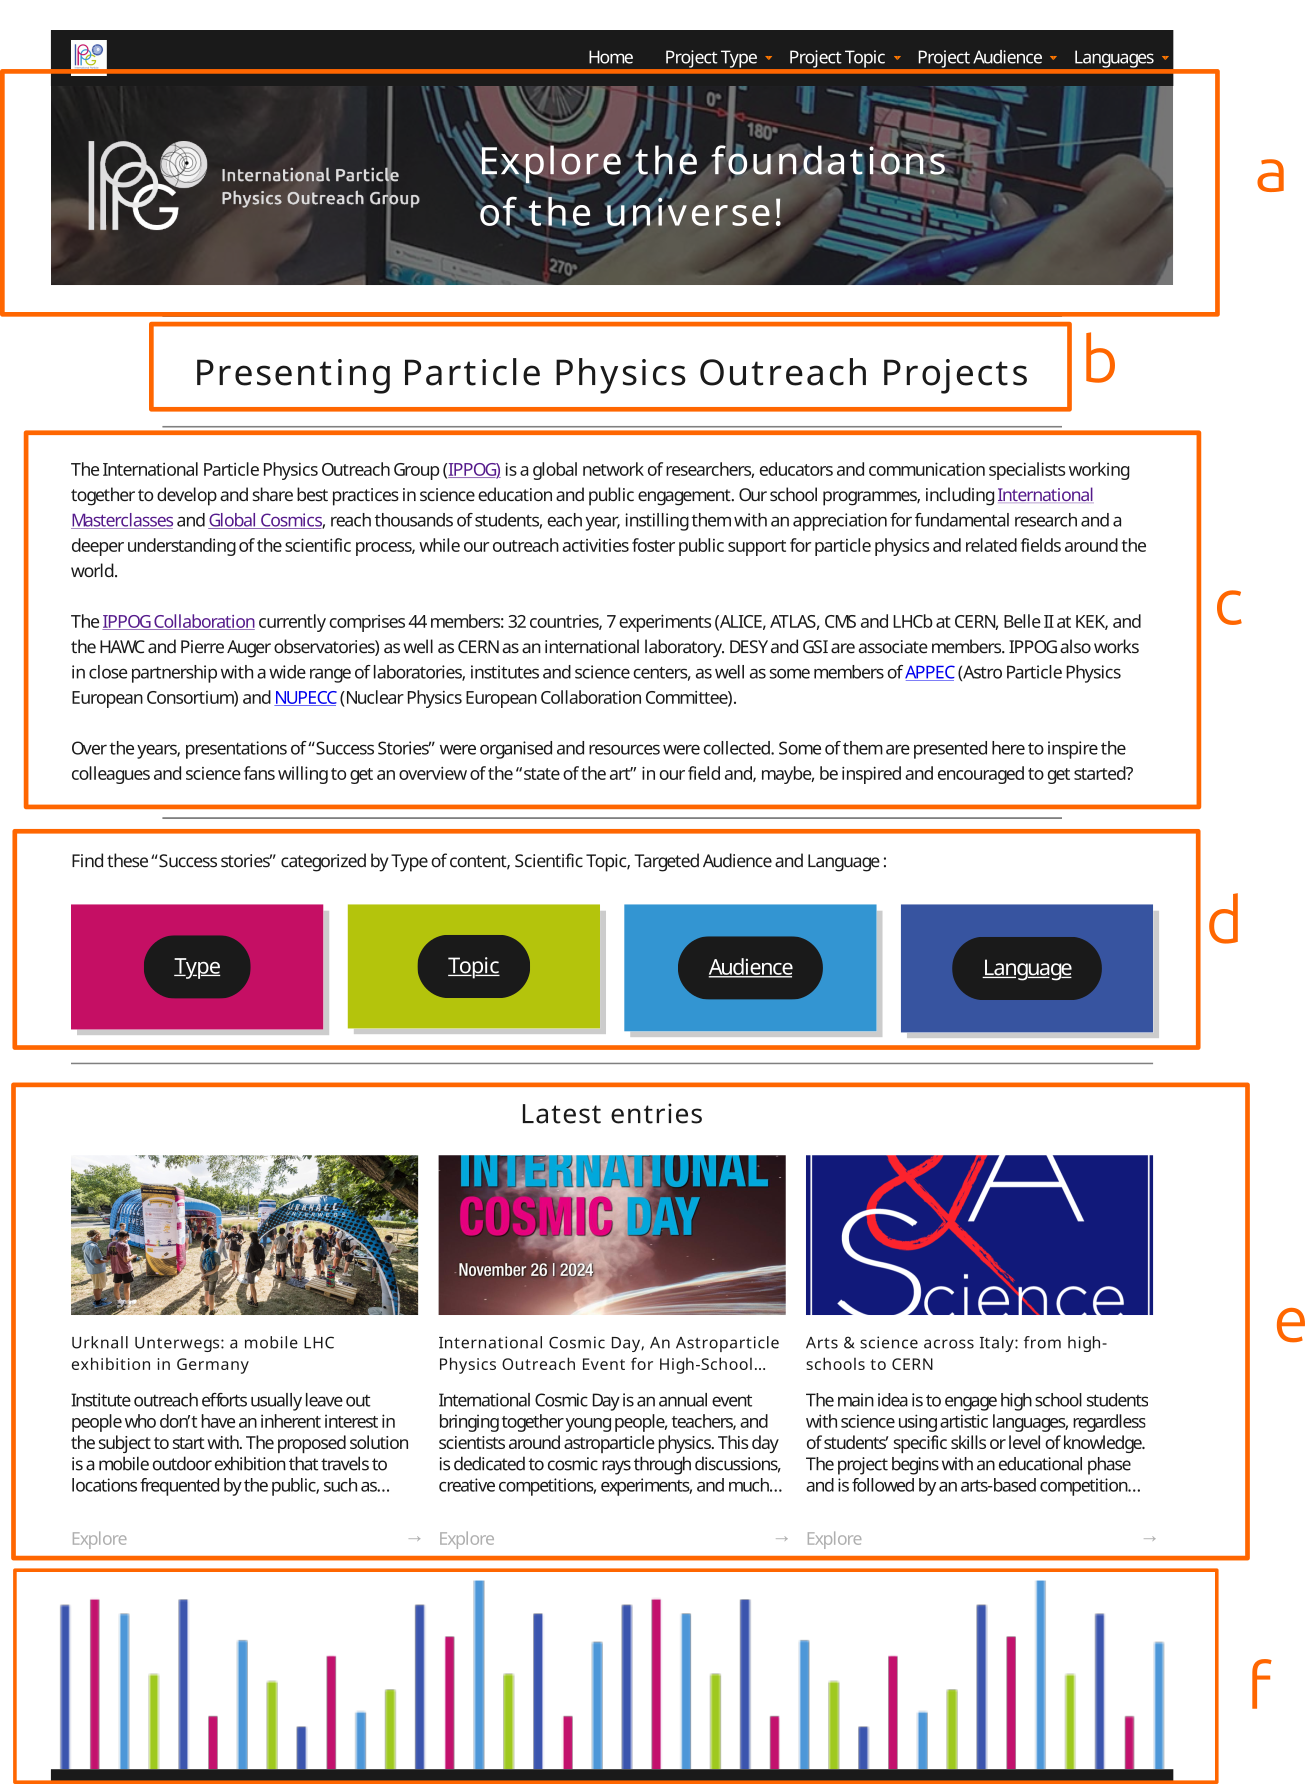
\includegraphics[width=\linewidth]{Image/Architecture/home_page.png}
    \caption{Website Home page}
    \label{fig:home_page}
\end{figure}

\newpage
\section{Menus}\label{sec:structure_menus}

Menus can be displayed in 2 locations: 
\begin{itemize}
    \item Header Navigation: at the top of the website
    \item Footer Navigation: at the bottom of the website, the footer is separated into 3 columns
\end{itemize}

\bigskip 

The website is using 3 menus (Fig. \ref{fig:menus}): 

\subsection*{a. CERN \& You}
This is the classic CERN menu displayed in all CERN websites. It is not displayed at the moment because it is not relevant for the collaboration.
/!\textbackslash \ It may automatically come back when the WordPress structure is updated.

\subsection*{b. General Information}
This menu gives further information about IPPOG and the website. 
\begin{itemize}
    \item A first link "Custom Link Brought to you by the IPPOG collaboration, on behalf of the Particle Physics outreach community." leads to the FAQ (Section \ref{ssec:structure_FAQ}),
    \item The second link "Further details on the categorization." leads to the explanation of the tags (Section \ref{ssec:structure_Categorization}).
\end{itemize}

\subsection*{c. Main Navigation}
The main navigation menu includes links to: 
\begin{itemize}
    \item the Home page (Sec. \ref{sec:structure_home_page})
    \item the different pages related to meta-categories: Project Type / Project Topic / ... (Sec. \ref{sec:structure_metacategories}). By passing the mouse over the categories name, the user can make a scroll-down menu, detailing the different category's pages: Universe / Matter \& Forces / ... (Sec. \ref{sec:structure_categories}).
\end{itemize}

\begin{figure}[p]
    \centering
    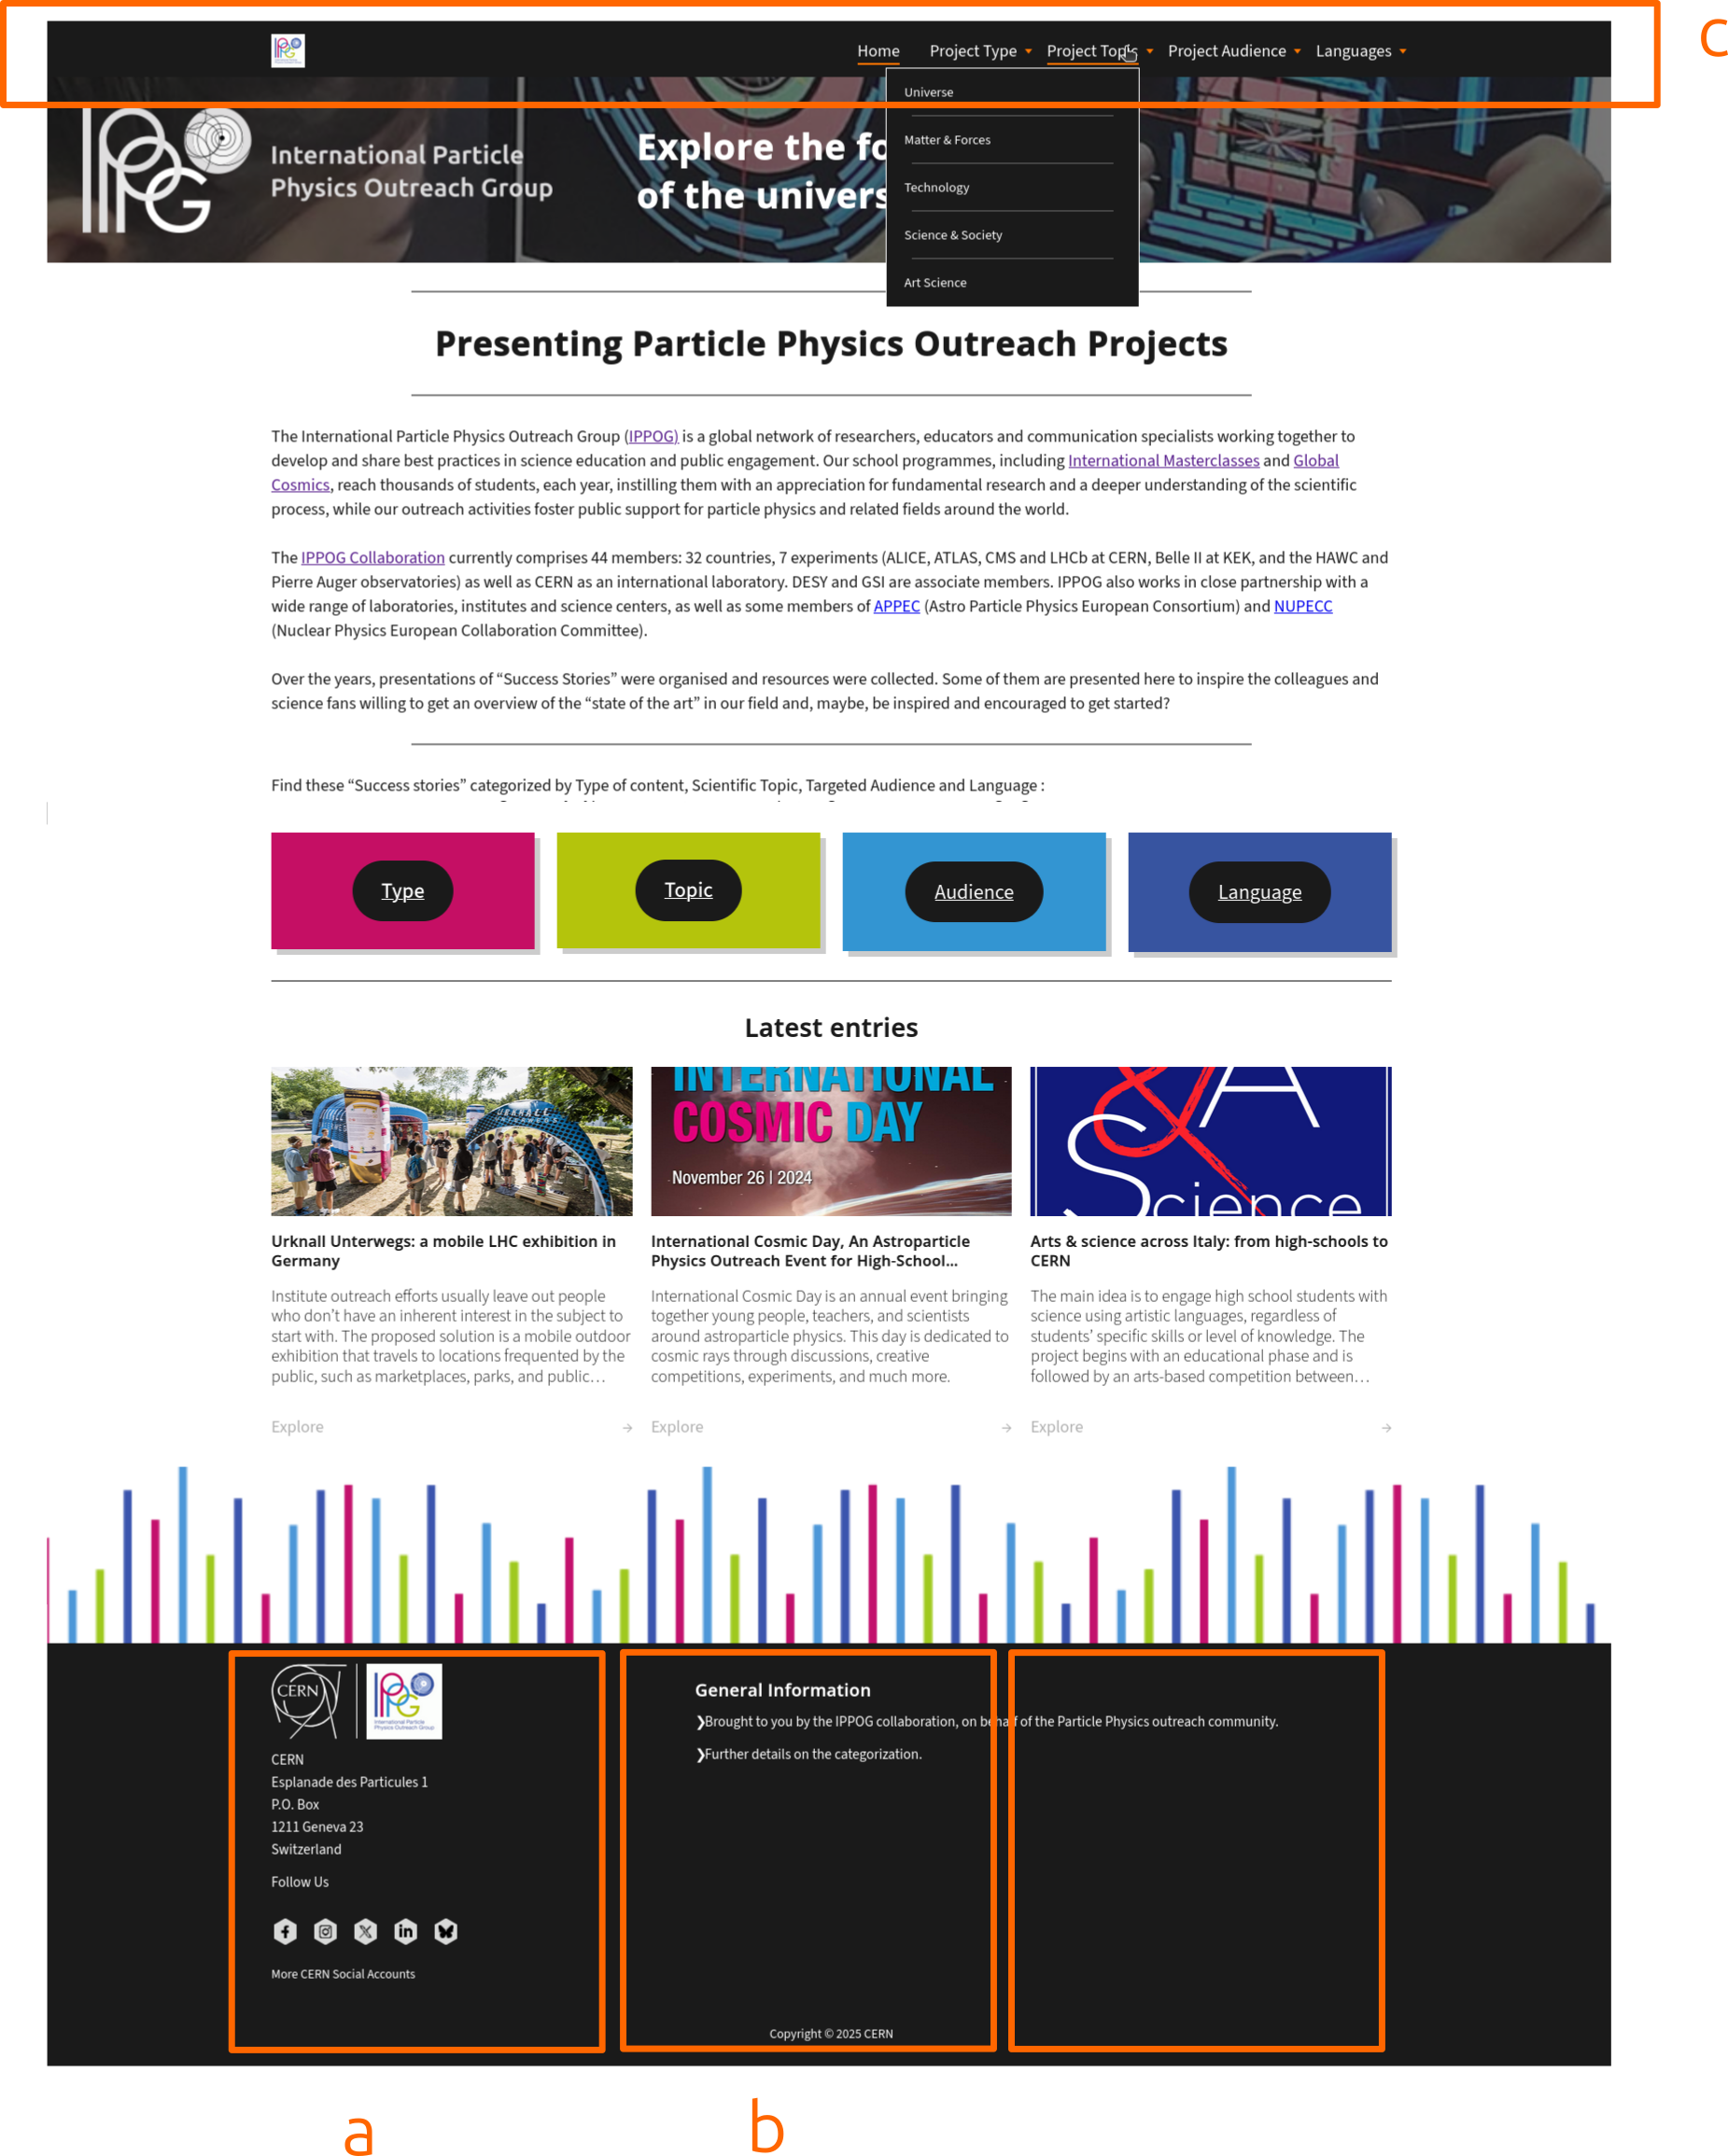
\includegraphics[width=\linewidth]{Image/Architecture/menus.png}
    \caption{Website menus}
    \label{fig:menus}
\end{figure}

\newpage
\section{Meta-Categories pages}\label{sec:structure_metacategories}

The Meta-Categories pages (Fig. \ref{fig:structure_metacategory}) display all categories related to the meta-category and the last three projects uploaded for each category.

\subsection*{a. IPPOG color chart}
[Cover block] including one of the colors of the IPPOG's color chart.

\subsection*{b. Title}
[H1 Title block]: Either "Project Type" / "Project Topic" / "Project Audience".

\subsection*{c. List of categories}
[Buttons block] leading to the categories pages nested within [Cover block] in a [Columns block].

\subsection*{d. Latest updated projects for each category}
[Group block] For each category\footnote{Except for the "Language" meta-category that doesn't have this part.}. The block contains: 
\begin{itemize}
    \item a [Cover block] including one of the colors of the IPPOG's color chart,
    \item a [H2 Title block] "Latest projects for" followed by the name of the category,
    \item a [Paragraph block] introducing the category,
    \item a [News block] displaying the 3 latest articles uploaded in the relative category.
\end{itemize}

\begin{figure}[p]
    \centering
    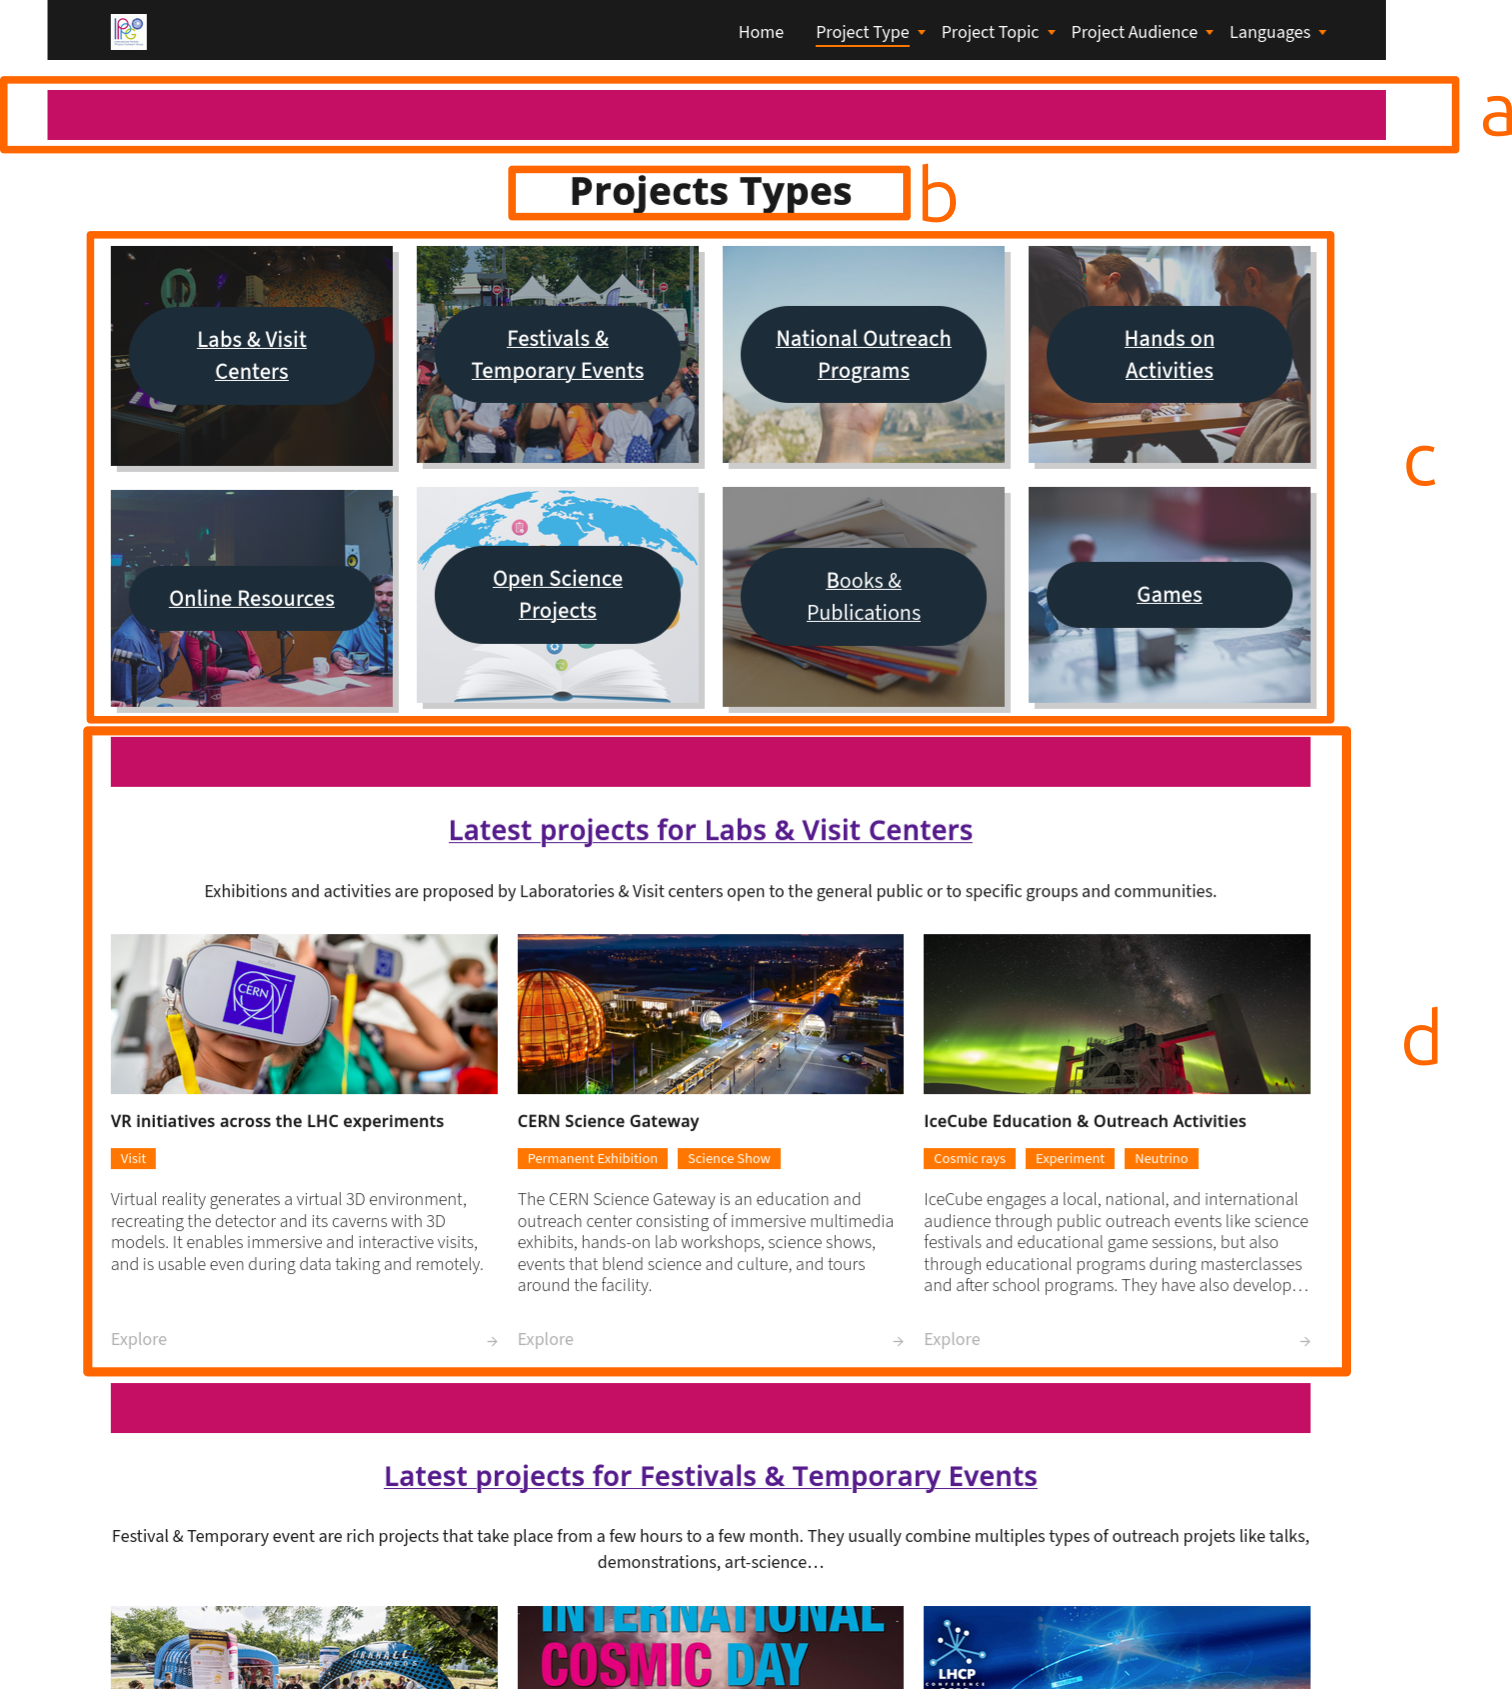
\includegraphics[width=\linewidth]{Image/Architecture/structure_types.png}
    \caption{Meta-categories pages (example of the "Projects Types" page)}
    \label{fig:structure_metacategory}
\end{figure}

\newpage

\section{Categories pages}\label{sec:structure_categories}

The Categories pages (Fig. \ref{fig:structure_category}) display all projects related to the category. The "Language" categories are a bit different and will be developed in more details in Sec. \ref{sec:structure_language}.

\subsection*{a. Category's banner}
[Cover block] including a [H1 Title block] with the name of the Category over a picture illustrating it.

\subsection*{b. Introduction}
[Paragraph block] introducing the category.

\subsection*{c. Tags}
[Paragraph block] introducing the tags followed by [Buttons block] leading to the automatically produced tags pages (Sec. \ref{sec:structure_auto})

\subsection*{d. Projects}
[News block] displaying all projects with the related category.

\begin{figure}[p]
    \centering
    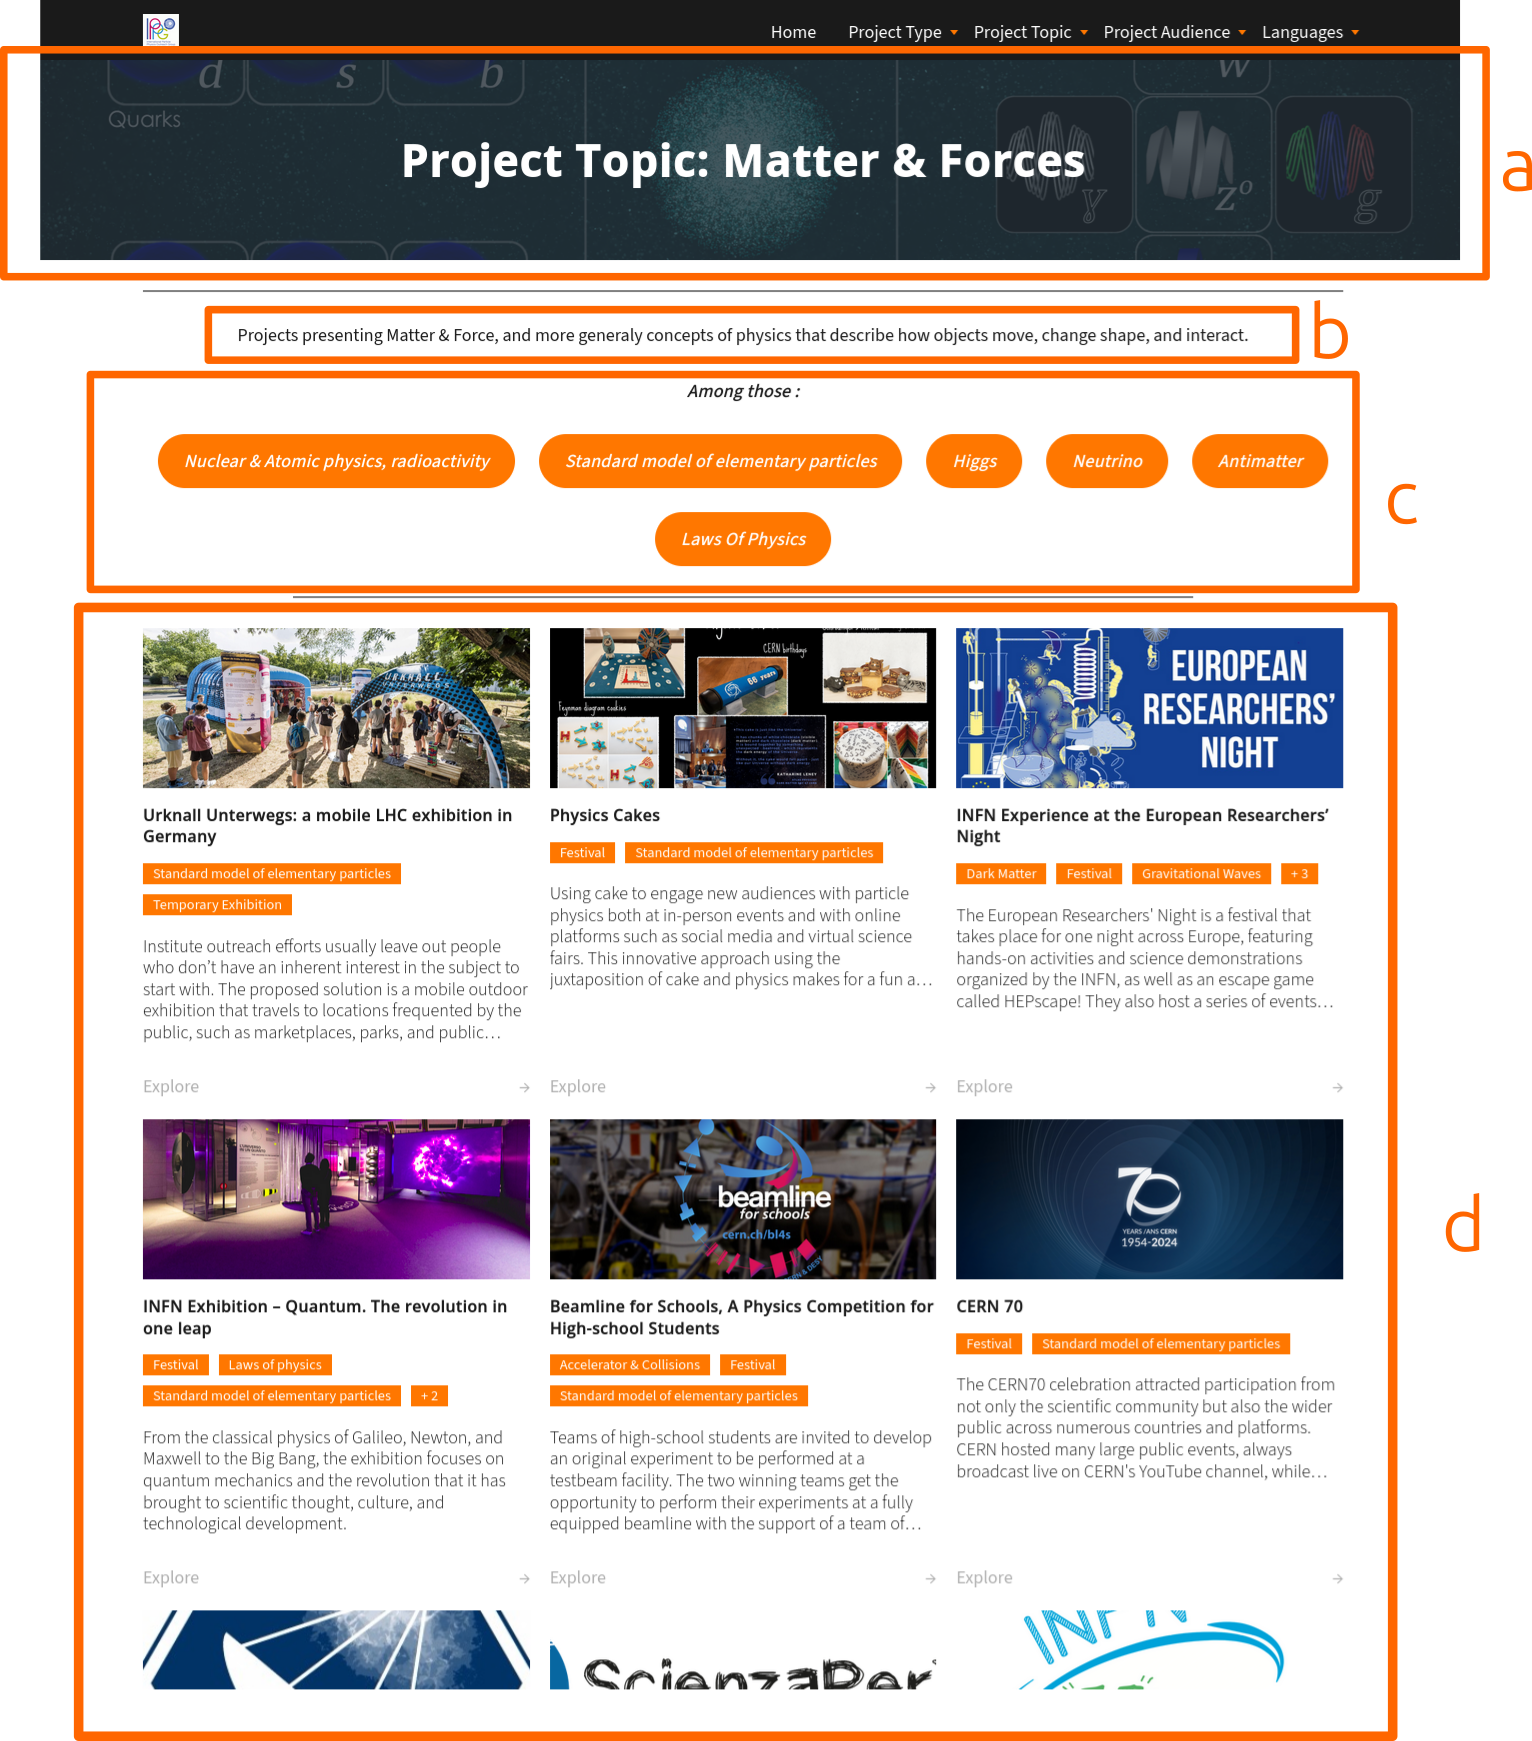
\includegraphics[width=\linewidth]{Image/Architecture/structure_category.png}
    \caption{Categories pages (example of the "Matter \& Forces" page)}
    \label{fig:structure_category}
\end{figure}
\newpage

\section{Languages Categories pages}\label{sec:structure_language}

The language categories (Fig. \ref{fig:structure_language}) are a bit different from other categories. As it aims to form discussion groups, these pages have a strong focus on the countries. Also, all these pages are translated into their own language.

\subsection*{a. Title}
[H1 Title block] with the name of the relative language.

\subsection*{b. Introduction}
[Paragraph block] introducing the members of the collaboration related to the language.

\subsection*{c. IPPOG members}
[Paragraph block] followed by a [List block] listing the representatives of the member countries with a link leading to the IPPOG general website.

\subsection*{d. Countries participating in Masterclass}
[Paragraph block] followed by a [List block] listing the countries (members of IPPOG or not) participating in International Physics Masterclass.

\subsection*{e. Projects}
[News block] displaying all projects with the related language.

\begin{figure}[p]
    \centering
    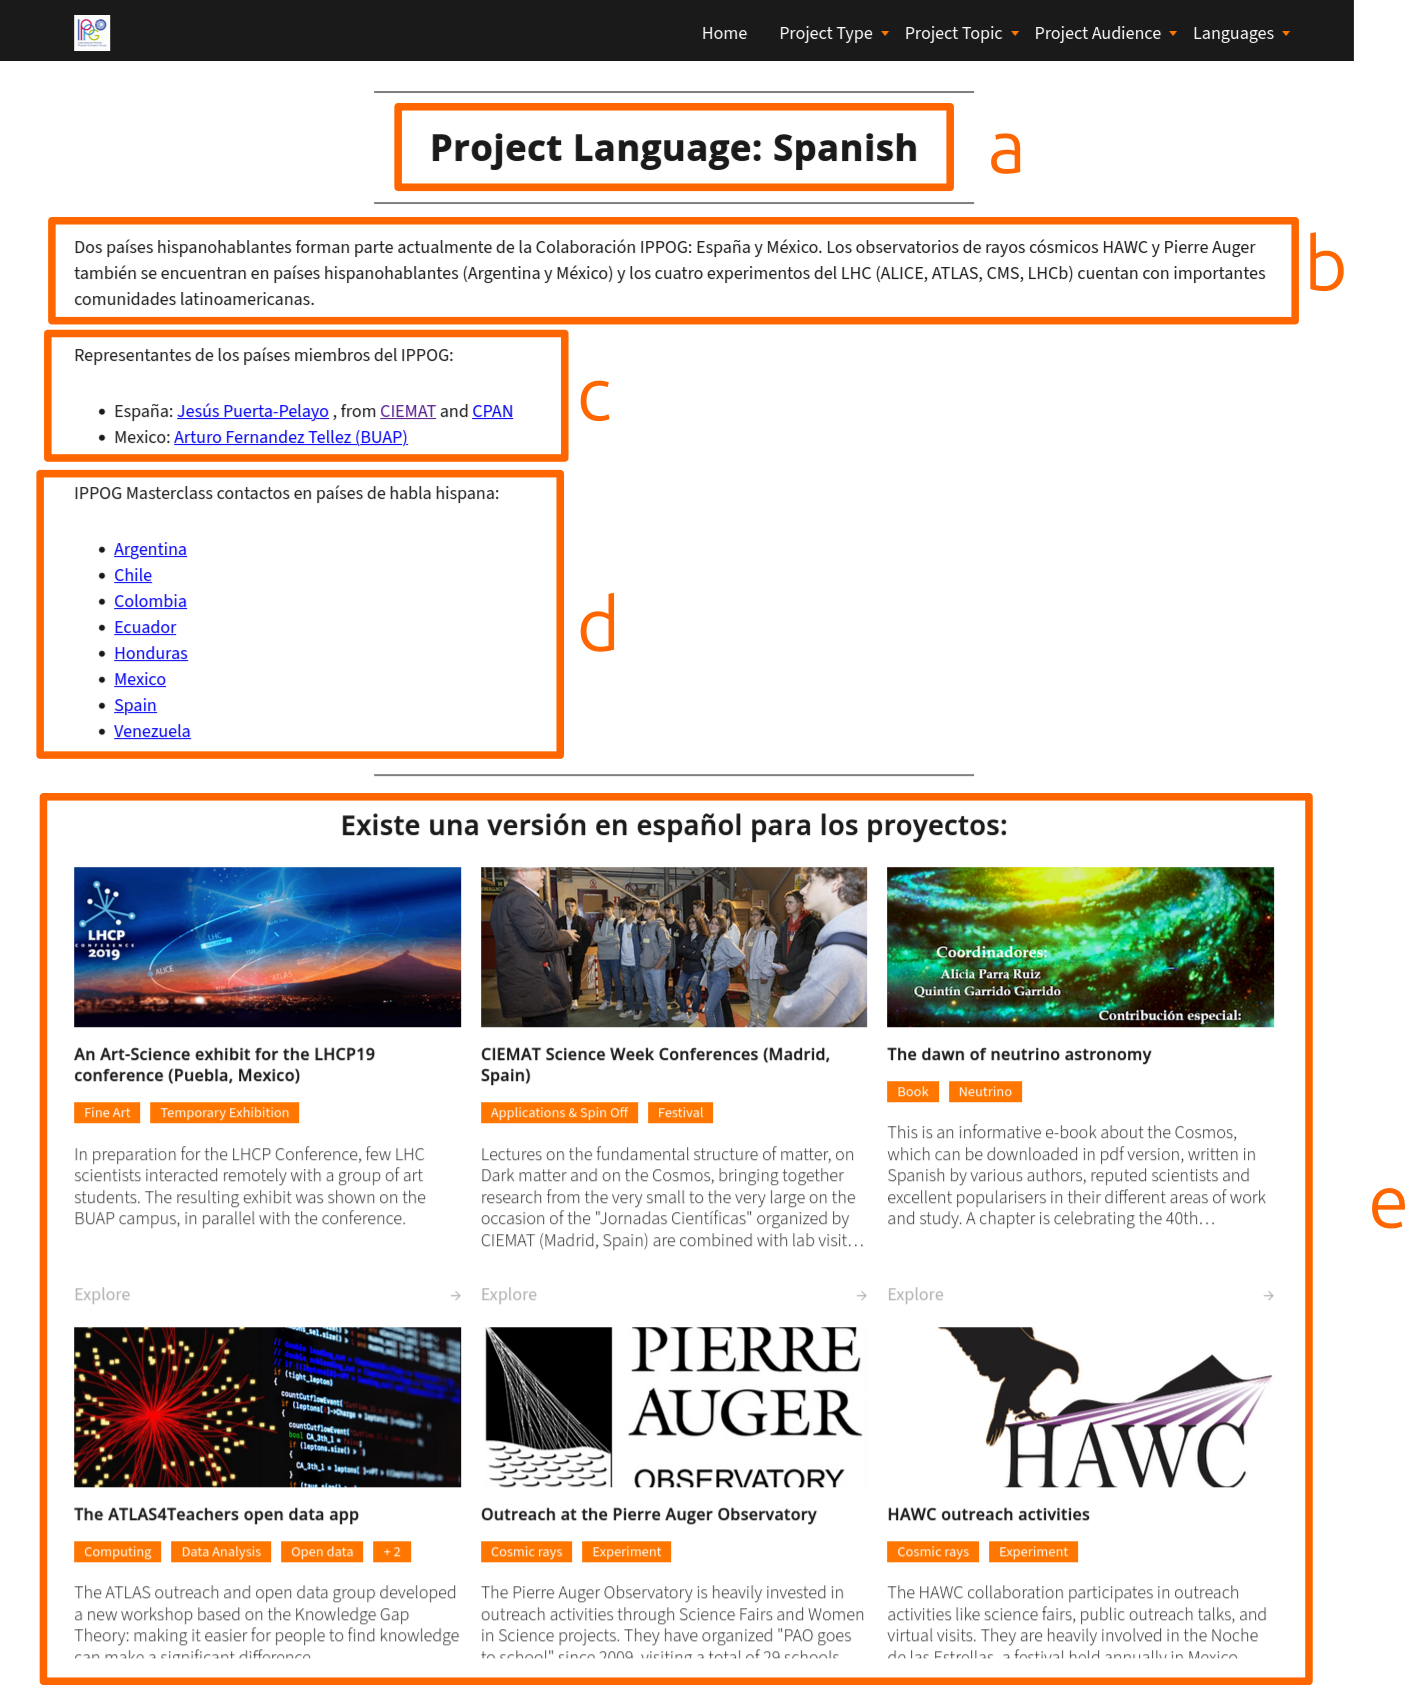
\includegraphics[width=\linewidth]{Image/Architecture/structure_language.png}
    \caption{Language category pages (example of the "Spanish" page)}
    \label{fig:structure_language}
\end{figure}
\newpage

\section{Projects Posts}\label{sec:structure_post}

The Posts (Fig. \ref{fig:structure_post}) present all information relevant to one project. All data are extracted from the database.

\subsection*{a. Title \& Image}
[Media \& Text block] made of the [Featured Image block] of the post on the right, and the [H1 Title block] of the post on the left. There can also be a [H2 Title block] working as a subtitle below the title.

\subsection*{b. Credit for the image}
[Paragraph block] crediting the author of the featured image, aligned on the right.

\subsection*{c. Abstract}
[H2 Title block] "Abstract" followed by a [Paragraph block] briefly describing the project.

\subsection*{d. Presentation slides}
[List block] linking to the presentation of the project during a conference or a meeting.

\subsection*{e. Authors}
[H2 Title block] "Contact" followed by a [Paragraph block] "Authors: " and a [List block] listing the authors of the project and their affiliations.

\subsection*{f. Related IPPOG members}
[Paragraph block] "Related IPPOG Collaboration members:" followed by a [List block] listing the IPPOG members relevant for the project, and linking to the general IPPOG website.

\subsection*{g. Public Contact}
[Paragraph block] "Contact:" followed by a [List block] with either an email or a link to a contact form to contact the authors of the project.

\subsection*{h. Status}
[H2 Title block] "Project status" followed by a [Paragraph block] describing the status of the project and the last time the post was updated.

\subsection*{i. Files \& Resources}
[H2 Title block] "Files \& Resources" followed by a [List block] linking to relevant resources.

\subsection*{j. Categories \& Tags}
[Categories block] and [Tags block] of the post linking to the automatically generated pages (Sec. \ref{sec:structure_auto}).

\begin{figure}[p]
    \centering
    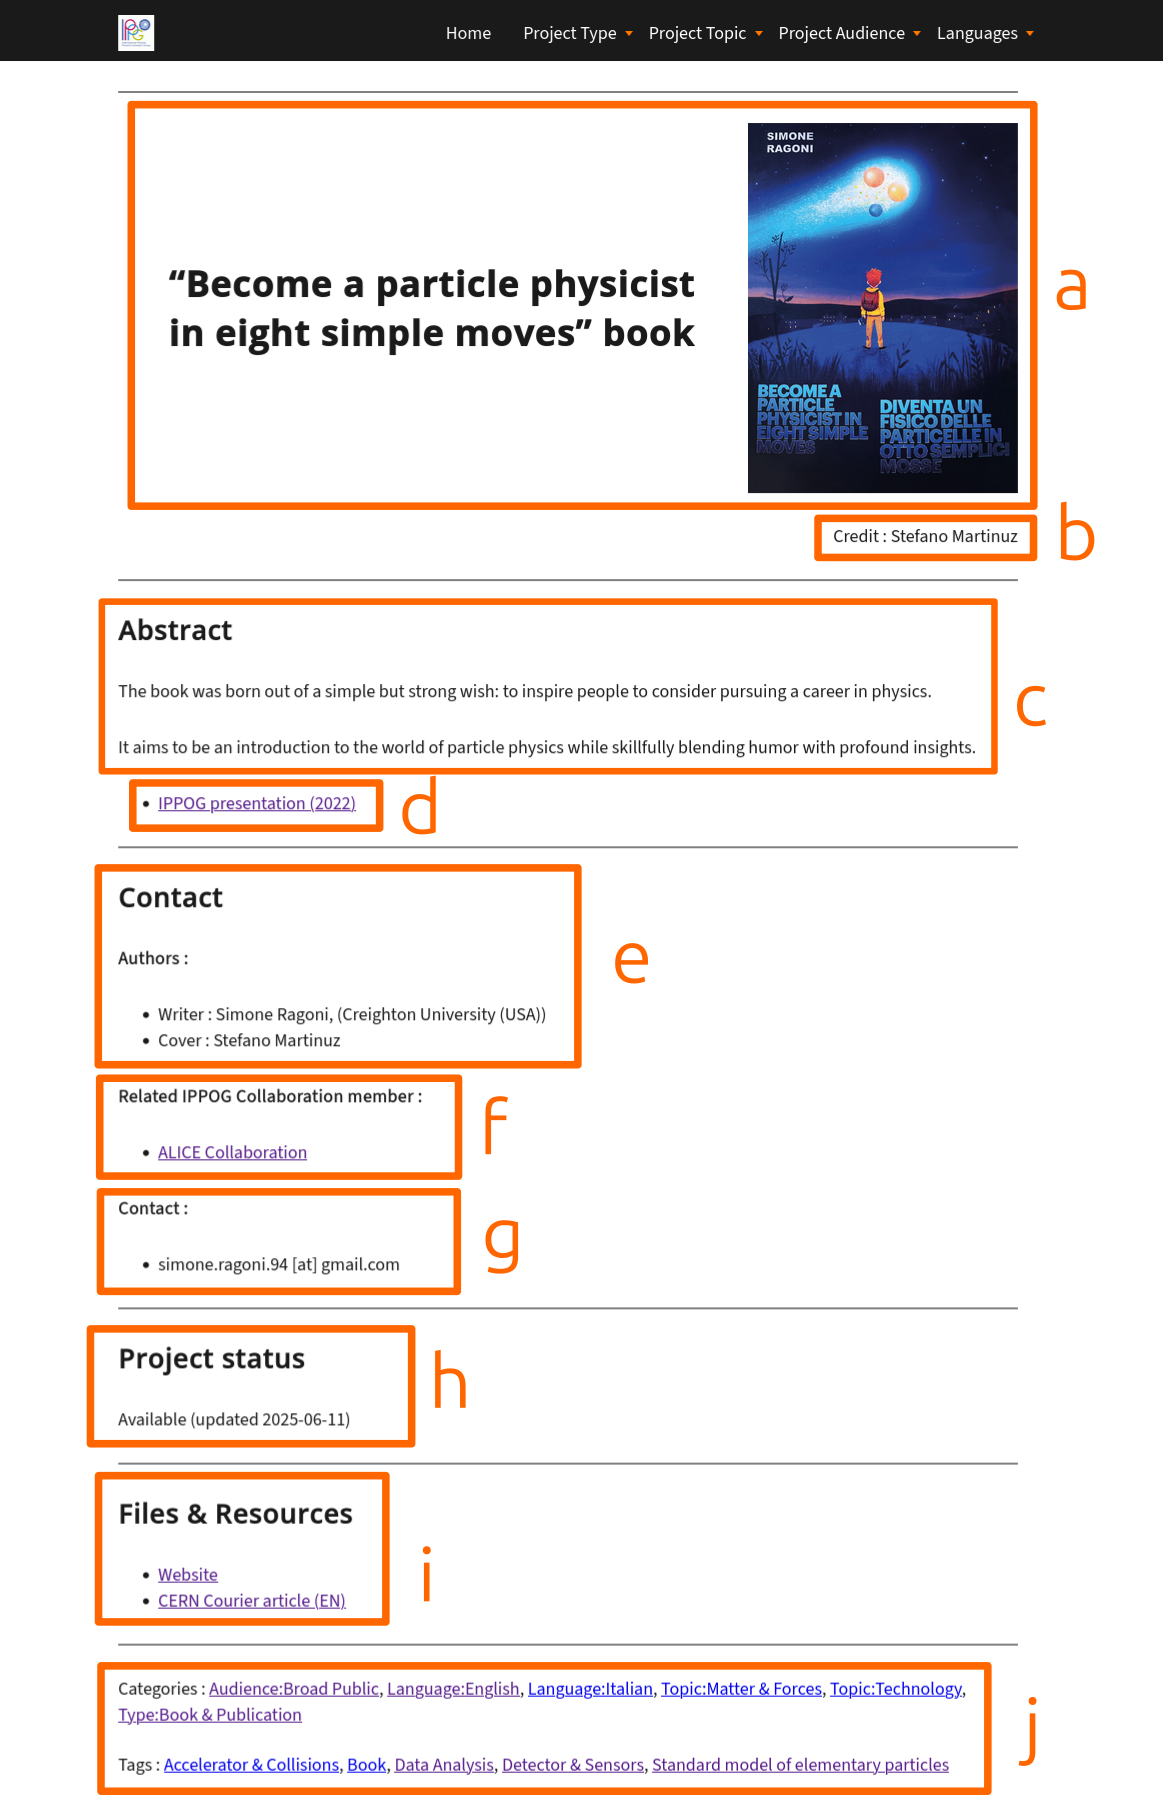
\includegraphics[width=.85\linewidth]{Image/Architecture/structure_project.png}
    \caption{Post pages (example of the “Become a particle physicist in eight simple moves book" post)}
    \label{fig:structure_post}
\end{figure}
\newpage

\section{Categories \& Tags automatic pages}\label{sec:structure_auto}

The WordPress automatically generates pages for each category and tag (Fig. \ref{fig:structure_auto}). Those pages can be accessed either through: 
\begin{itemize}
    \item the links in [News Blocks] (Fig. \ref{fig:structure_auto3}),
    \item at the top of category-specific pages (Fig. \ref{fig:structure_auto2}), or
    \item at the end of posts (Fig. \ref{fig:structure_auto1}).
\end{itemize}   
As they are generated automatically, they cannot be modified at the moment and, as such, they remain not very visually attractive. This is why the choice was made to create easier-to-navigate pages (Sec. \ref{fig:structure_category}).

\bigskip

\begin{figure}[th]
    \begin{subfigure}[c]{.5\textwidth}
        \centering
        \begin{subfigure}[t]{\textwidth}
            \centering
            
\includegraphics[width=\textwidth]{Image/Architecture/structure_auto1.png}
            \caption{at the end of posts}
            \label{fig:structure_auto1}
        \end{subfigure}
        
             
        \vspace{2cm}
        \begin{subfigure}[c]{\textwidth}
            \centering
            
\includegraphics[width=\textwidth]{Image/Architecture/structure_auto2.png}
            \caption{at the top of category-specific pages}
            \label{fig:structure_auto2}
        \end{subfigure}
    \end{subfigure}
    \hfill  % NOTE1: hfill moves horizontally stacked objects as far apart as it can
    \begin{subfigure}[c]{.4\textwidth}
        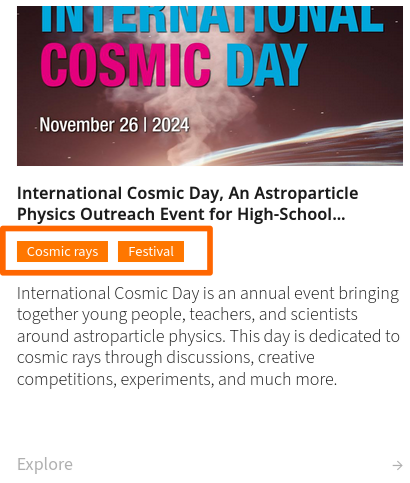
\includegraphics[width=\textwidth]{Image/Architecture/structure_auto3.png}
        \caption{in [News Blocks]}
        \label{fig:structure_auto3}
    \end{subfigure}
    \caption{Links to Categories \& Tags automatic pages}
\end{figure}

\begin{figure}[p]
    \centering
    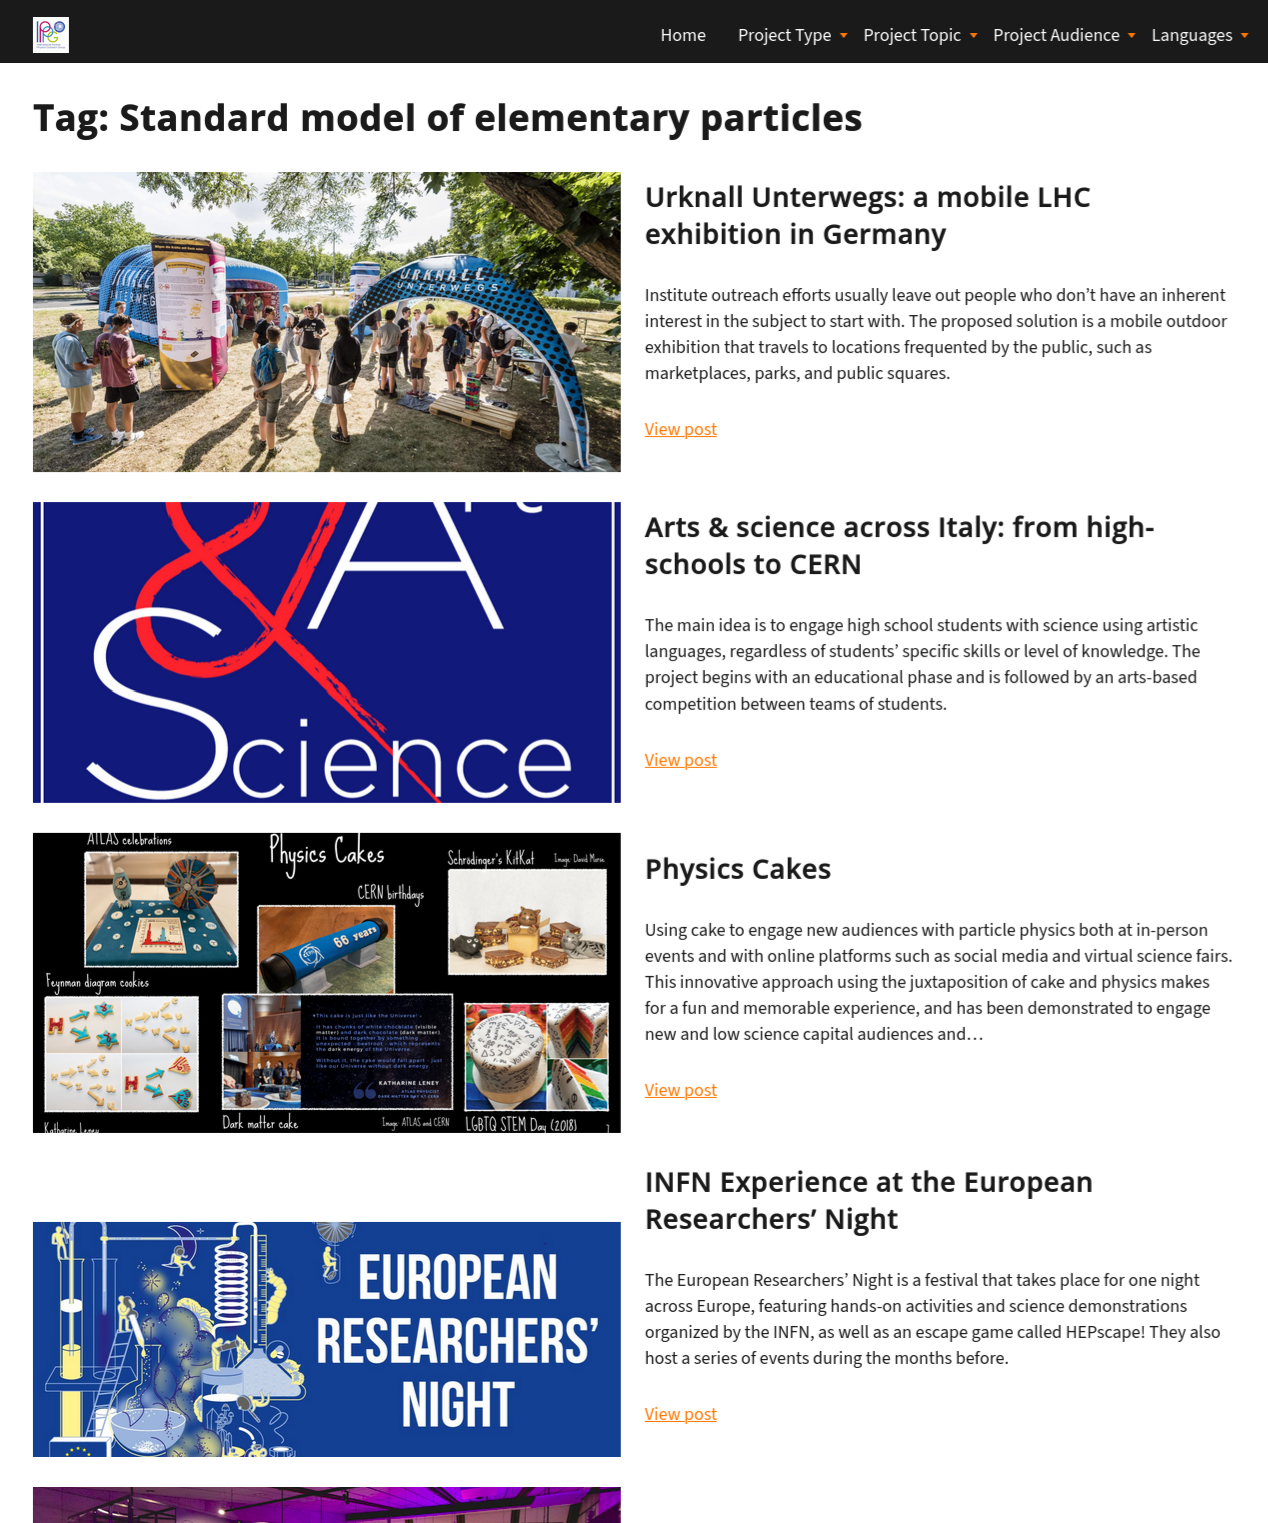
\includegraphics[width=\linewidth]{Image/Architecture/structure_auto.png}
    \caption{Categories \& Tags automatic pages}
    \label{fig:structure_auto}
\end{figure}

\newpage

\section{General Information}\label{sec:structure_genaralinfo}

The General Information menu (Fig. \ref{fig:structure_general_info}) links to two pages: a general description of the IPPOG Collaboration (Sec. \ref{ssec:structure_FAQ}) and the Taxonomy used in the website (Sec. \ref{ssec:structure_Categorization})

\smallskip

\begin{figure}[h!]
    \centering
    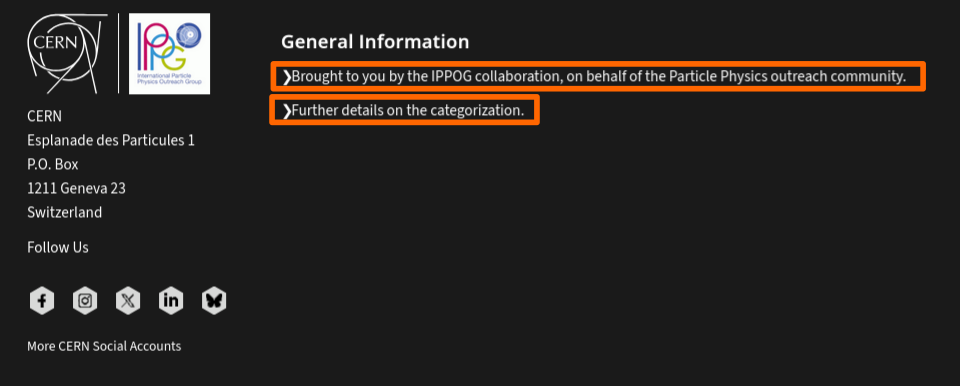
\includegraphics[width=.9\linewidth]{Image/Architecture/structure_general_info.png}
    \caption{General Information menu}
    \label{fig:structure_general_info}
\end{figure}

\subsection{FAQ}\label{ssec:structure_FAQ}

The FAQ page (Fig. \ref{fig:structure_faq}) gives a general description of the collaboration.

\subsubsection*{a. Presentation of the IPPOG}
This section presents the IPPOG collaboration, its goals, members, and a few relevant links.

\subsubsection*{b. Flagship activities of the IPPOG}
This section lists the current activities of the IPPOG collaboration.

\subsubsection*{c. Presentation of the Resource Portal}
This is a small presentation of the Resource Portal and why it was created.

\subsubsection*{d. Contact}
Link to the contact form.

\subsection{Categorization}\label{ssec:structure_Categorization}

This page (Fig. \ref{fig:structure_taxonomy}) gives a quick overview of the taxonomy used to classify the projects on the website.

\subsubsection*{a. Introduction}
This section gives a small introduction to the taxonomy.

\subsubsection*{b. Taxonomy}
This is the infographic available in Fig \ref{fig:Topics_category} \& \ref{fig:Types_category}. These are created using the FraMindmap software (Sec. \ref{sec:map}).

\begin{landscape}
    
    \begin{figure}[p]
        \centering
        \begin{subfigure}[c]{.5\textwidth}
            \centering
            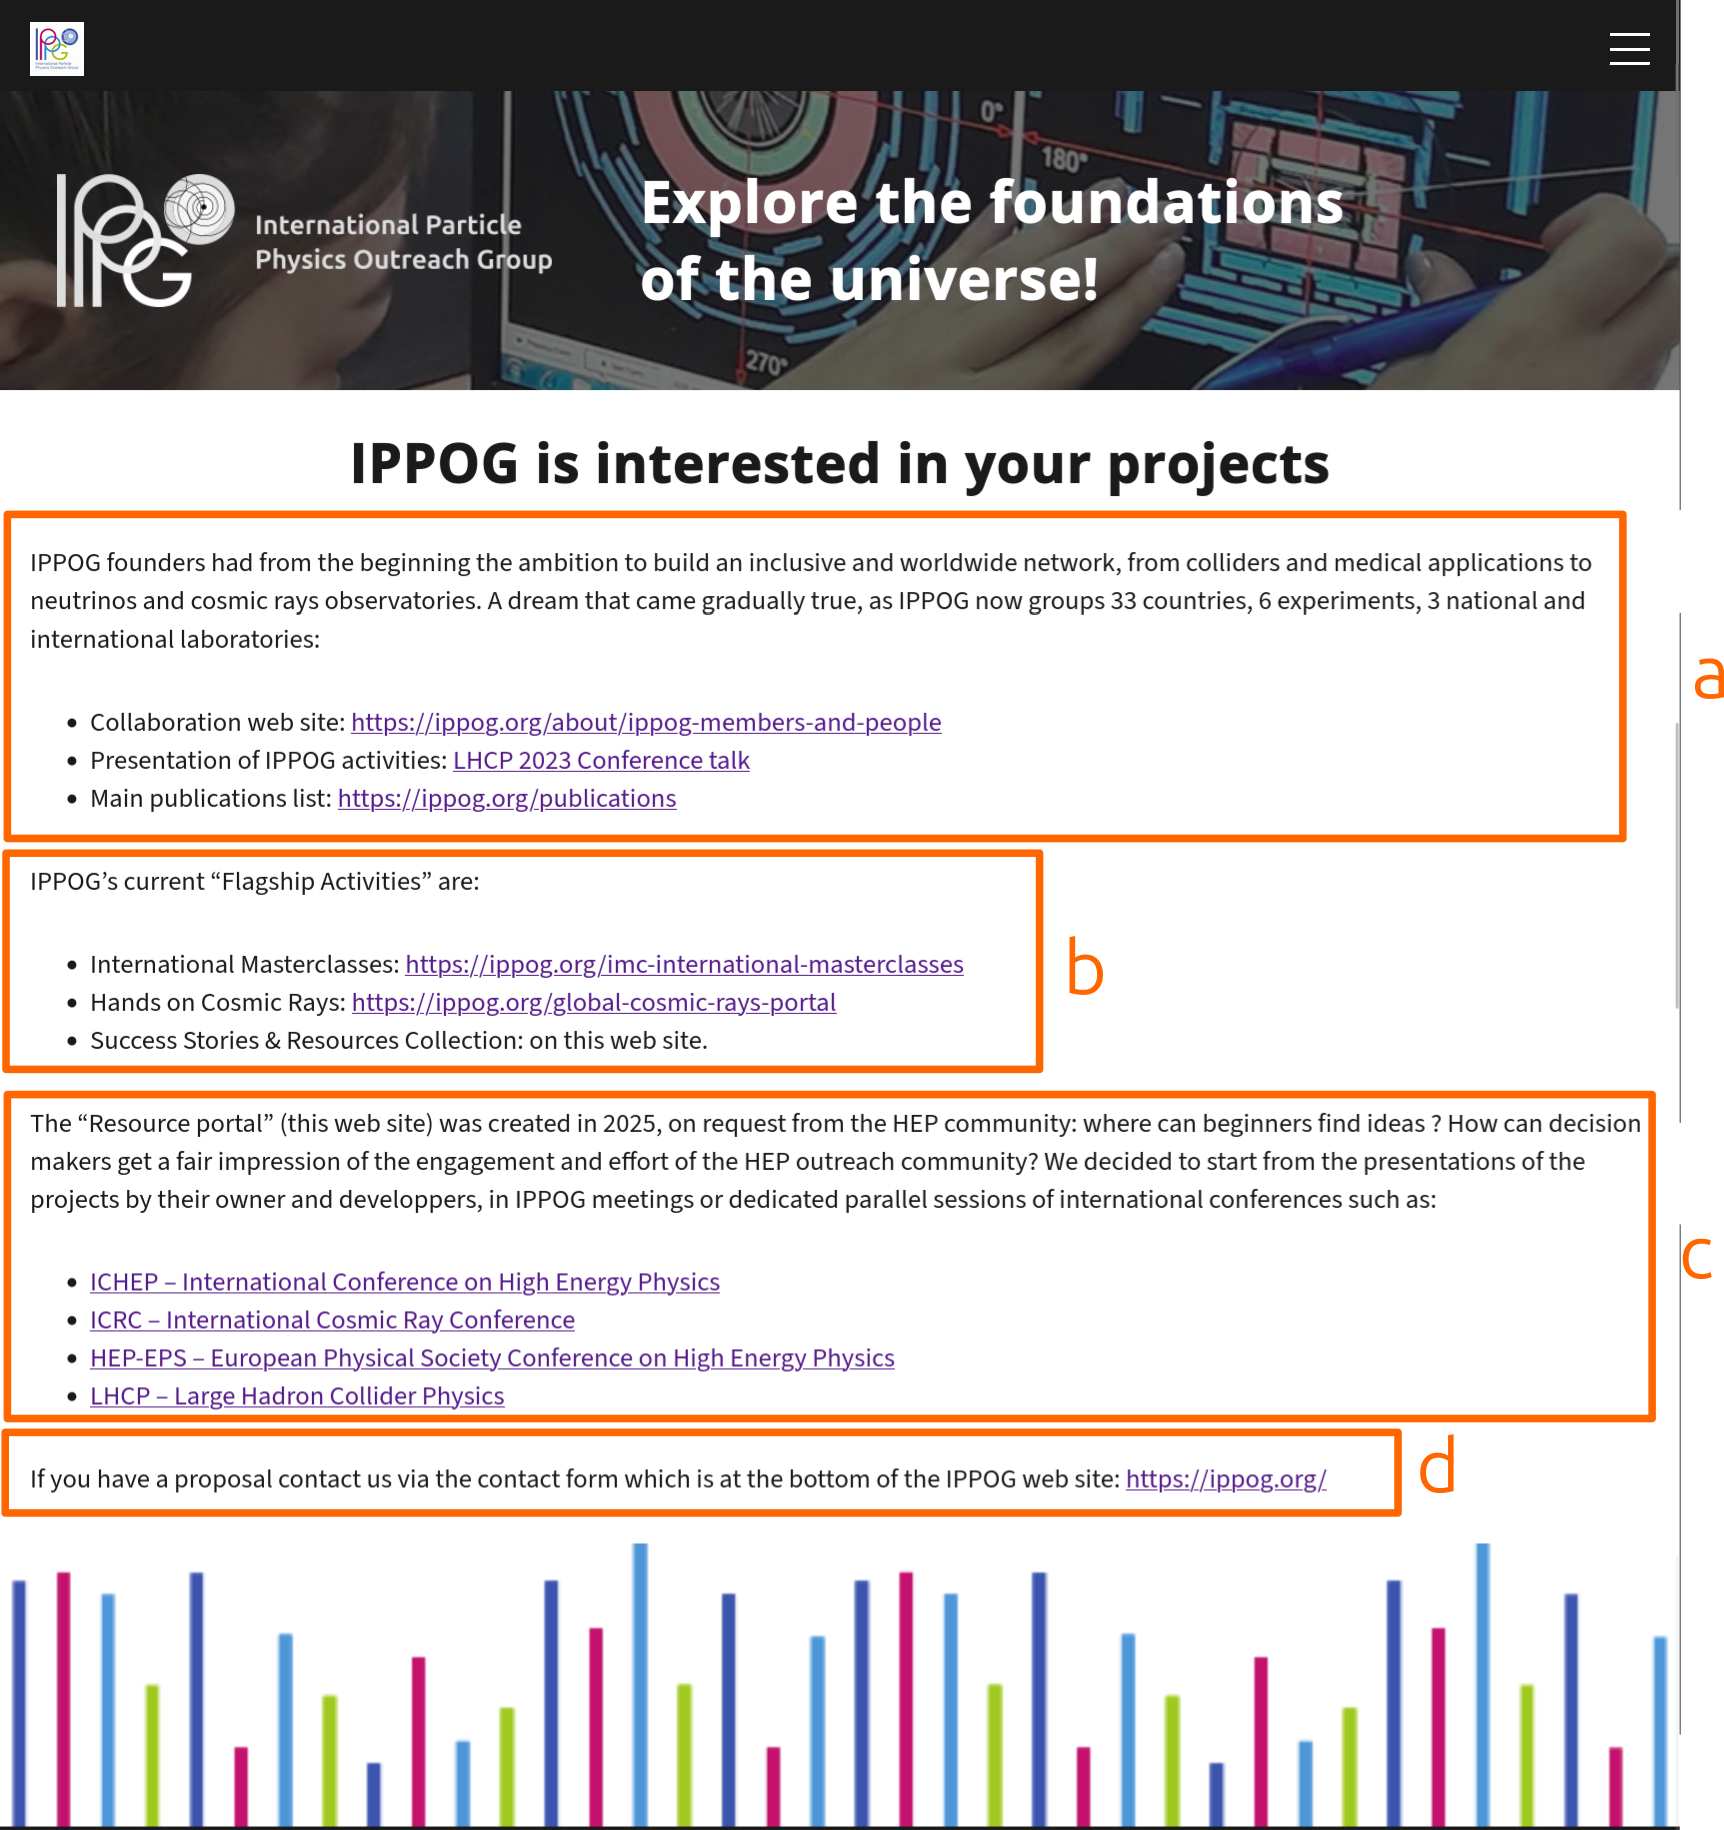
\includegraphics[width=1.2\linewidth]{Image/Architecture/structure_faq.png}
            \caption{FAQ page}
            \label{fig:structure_faq}
        \end{subfigure}
        \hspace{3cm}
        \begin{subfigure}[c]{.5\textwidth}
            \centering
            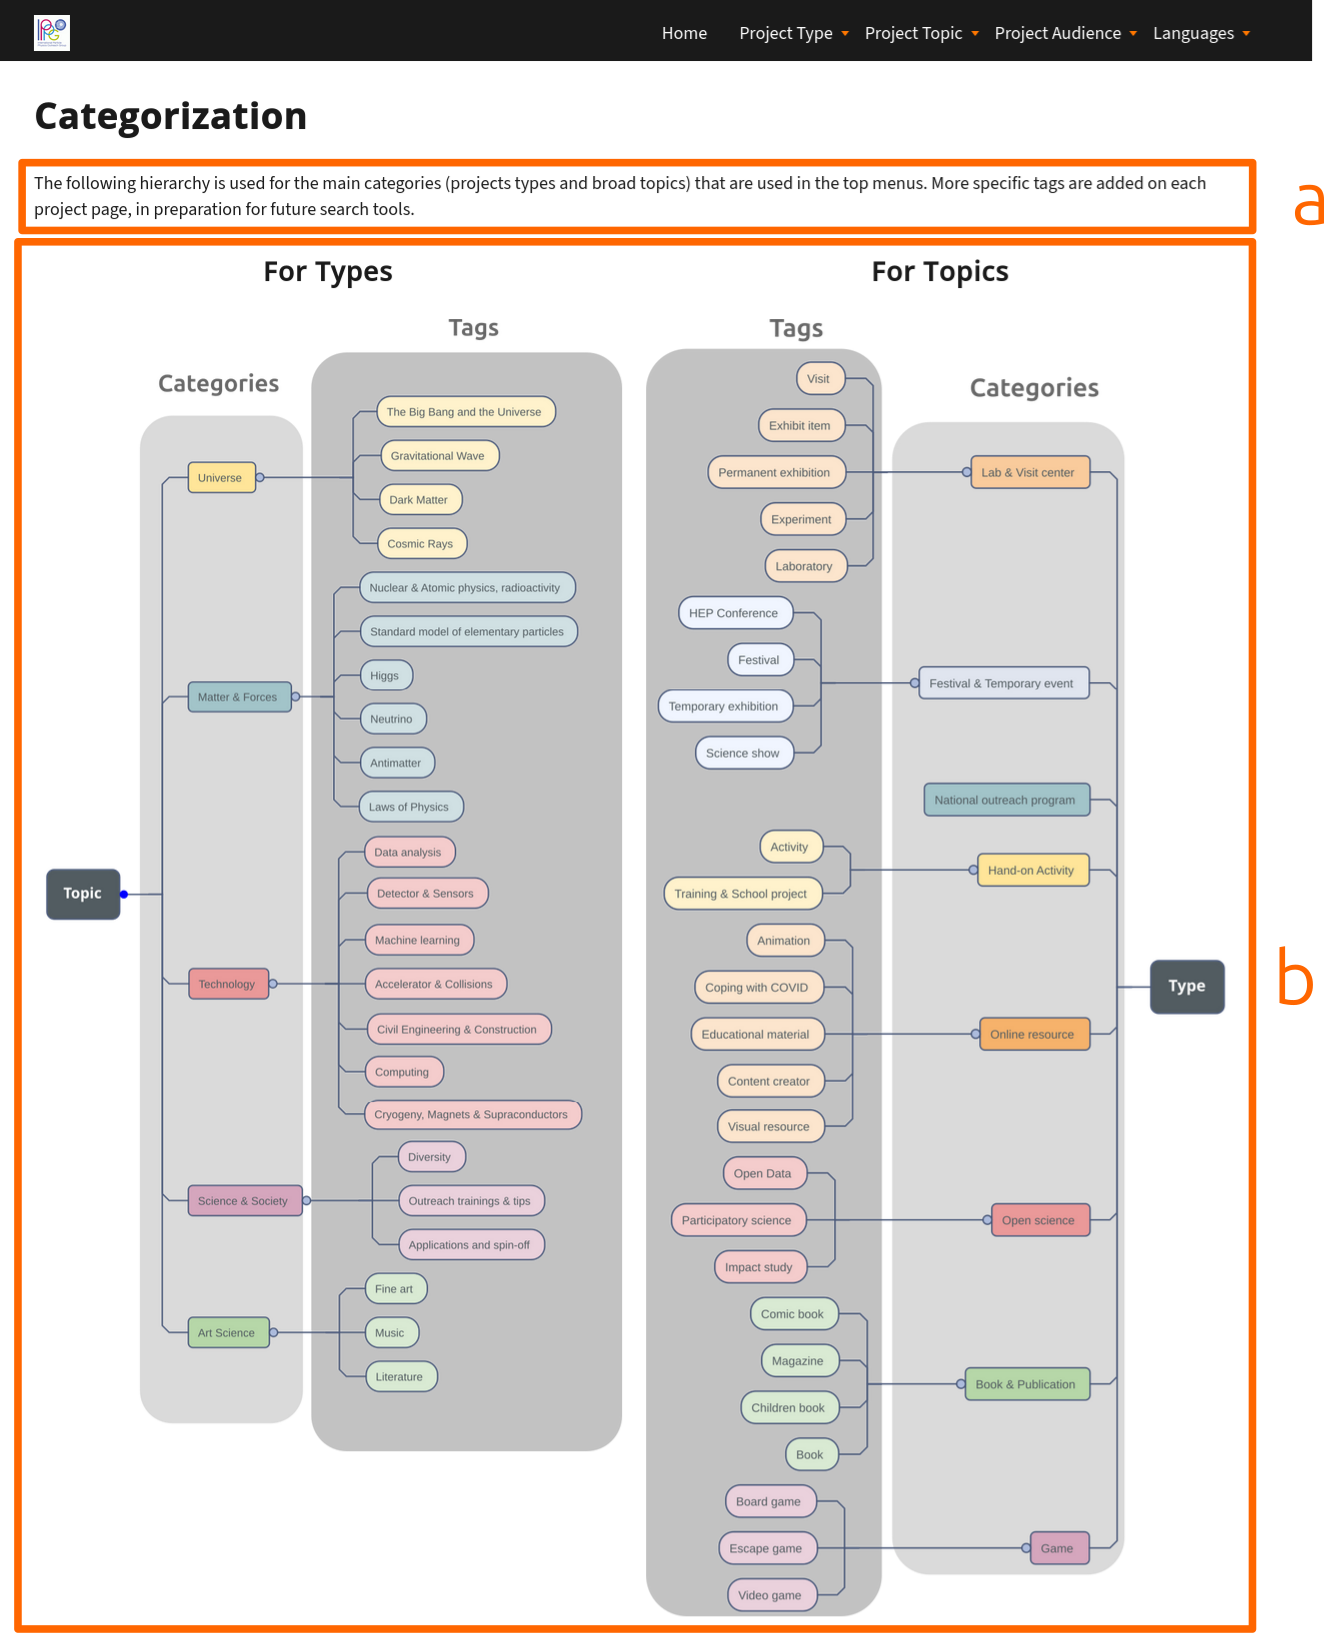
\includegraphics[width=1.2\linewidth]{Image/Architecture/structure_taxonomy.png}
            \caption{Taxonomy page}
            \label{fig:structure_taxonomy}
        \end{subfigure}
        \label{fig:gform}
        \caption{General Information menu}
    \end{figure}

\end{landscape}